\documentclass[10pt,aspectratio=169]{beamer}

\usetheme{Madrid}
\usefonttheme{professionalfonts}
\usecolortheme{default}

\usepackage{amsmath,amssymb,bm}
\usepackage{tikz}
\usepackage{booktabs}
\usepackage{listings}
\usepackage{xcolor}
\usepackage{colortbl}

\usetikzlibrary{positioning,arrows.meta,calc,fit}

\definecolor{myblue}{RGB}{31,78,121}
\definecolor{deepblue}{RGB}{20,55,95}
\definecolor{blockblue}{RGB}{42,92,145}
\definecolor{softblue}{RGB}{225,235,245}
\definecolor{mygreen}{RGB}{40,130,90}
\definecolor{myred}{RGB}{180,60,60}

\setbeamercolor{background canvas}{bg=white}
\setbeamercolor{normal text}{fg=black,bg=white}

\setbeamercolor{frametitle}{fg=white,bg=myblue}
\setbeamerfont{frametitle}{series=\bfseries}

\setbeamercolor{title}{fg=white}
\setbeamercolor{subtitle}{fg=white}
\setbeamercolor{author}{fg=black}
\setbeamercolor{date}{fg=black}

\setbeamercolor{structure}{fg=myblue}
\setbeamercolor{item}{fg=myblue}
\setbeamercolor{subitem}{fg=myblue}
\setbeamercolor{enumerate item}{fg=myblue}

\setbeamercolor{block title}{fg=white,bg=myblue}
\setbeamercolor{block body}{fg=black,bg=softblue}

\setbeamercolor{palette primary}{fg=white,bg=myblue}
\setbeamercolor{palette secondary}{fg=white,bg=deepblue}
\setbeamercolor{palette tertiary}{fg=white,bg=deepblue}
\setbeamercolor{palette quaternary}{fg=white,bg=myblue}

\setbeamertemplate{navigation symbols}{}

\setlength{\abovedisplayskip}{4pt}
\setlength{\belowdisplayskip}{4pt}
\setlength{\abovedisplayshortskip}{3pt}
\setlength{\belowdisplayshortskip}{3pt}
\arrayrulecolor{myblue}

\newcommand{\grad}[2]{\frac{\partial #1}{\partial #2}}
\newcommand{\adj}[1]{\bar{#1}}

\tikzset{
    var/.style={
        circle,
        draw=myblue,
        fill=white,
        thick,
        minimum size=0.72cm,
        inner sep=1pt,
        font=\small
    },
    op/.style={
        rectangle,
        draw=mygreen,
        fill=white,
        thick,
        rounded corners,
        minimum width=1.0cm,
        minimum height=0.58cm,
        inner sep=3pt,
        font=\small
    },
    arr/.style={->,thick,myblue,>=Latex},
    % barr/.style={<-,thick,myred,>=Latex}
    barr/.style={->,thick,myred,>=Latex}
}

\lstset{
    basicstyle=\ttfamily\footnotesize,
    breaklines=true,
    columns=fullflexible,
    frame=single,
    rulecolor=\color{myblue},
    backgroundcolor=\color{softblue},
    showstringspaces=false
}

\title{Computational Graphs and Automatic Differentiation}
\subtitle{The mechanics behind backpropagation}
\author{}
\date{}

\begin{document}

\begin{frame}
\titlepage
\end{frame}
\begin{frame}{Session map}
\begin{enumerate}
    \item Computational graphs as data-flow programs
    \item Forward pass: evaluate values
    \item Backward pass: send gradients
    \item Gradient accumulation at branches
    \item Reverse-mode autodiff
    \item PyTorch autograd mental model
\end{enumerate}

\vspace{0.4cm}

\[
\boxed{
\text{Backpropagation} =
\text{reverse-mode autodiff on a computational graph}
}
\]
\end{frame}

\begin{frame}[t]{Why computational graphs?}
A neural network is not one giant formula in memory.

It is a sequence of simple operations:

\[
\text{matmul}
\rightarrow
\text{add}
\rightarrow
\text{activation}
\rightarrow
\cdots
\rightarrow
\text{loss}
\]

A computational graph records:

\begin{itemize}
    \item what was computed,
    \item which values were used,
    \item which operation produced each value,
    \item how gradients should flow backward.
\end{itemize}
\end{frame}

\begin{frame}[t]{A function as a program}
Consider:

\[
L=(xy+x)^2
\]

A program evaluates it as small steps:

\begin{columns}[T]
\column{0.32\textwidth}
\begin{block}{Step 1}
\[
a=xy
\]
\end{block}

\column{0.32\textwidth}
\begin{block}{Step 2}
\[
b=a+x
\]
\end{block}

\column{0.32\textwidth}
\begin{block}{Step 3}
\[
L=b^2
\]
\end{block}
\end{columns}

\vfill

Each step becomes one operation in the graph.
\end{frame}

\begin{frame}[t]{Computational graph for \(L=(xy+x)^2\)}
\centering

\resizebox{0.78\textwidth}{!}{
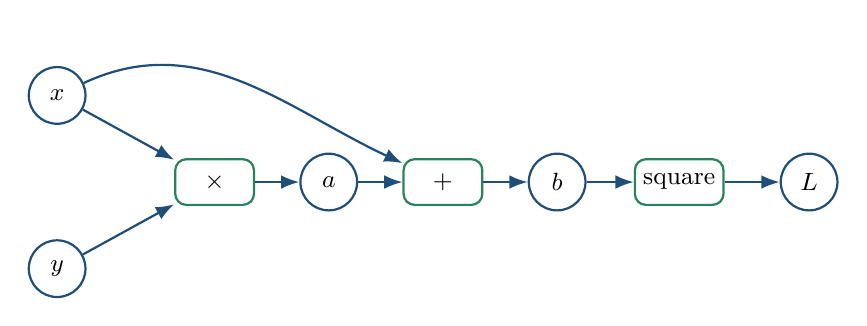
\begin{tikzpicture}
\node[var] (x) at (0,1.1) {$x$};
\node[var] (y) at (0,-1.1) {$y$};

\node[op]  (mul) at (2.0,0) {$\times$};
\node[var] (a) at (3.45,0) {$a$};

\node[op]  (add) at (4.9,0) {$+$};
\node[var] (b) at (6.35,0) {$b$};

\node[op]  (sq) at (7.9,0) {square};
\node[var] (L) at (9.55,0) {$L$};

\draw[arr] (x) -- (mul);
\draw[arr] (y) -- (mul);
\draw[arr] (mul) -- (a);
\draw[arr] (a) -- (add);
\draw[arr] (x) to[out=25,in=155] (add);
\draw[arr] (add) -- (b);
\draw[arr] (b) -- (sq);
\draw[arr] (sq) -- (L);
\end{tikzpicture}
}

\vspace{0.35cm}

\[
a=xy,\qquad b=a+x,\qquad L=b^2
\]

Notice that \(x\) is used twice.
\end{frame}

\begin{frame}[t]{What does an edge mean?}
\begin{columns}[T]
\column{0.48\textwidth}
\begin{block}{Forward direction}
An edge represents a dependency.

\[
u \rightarrow f \rightarrow v
\]

means:

\[
v=f(u)
\]
\end{block}

\column{0.48\textwidth}
\begin{block}{Backward direction}
During differentiation, information moves backward.

\[
\grad{L}{v}
\rightarrow
\grad{L}{u}
\]
\end{block}
\end{columns}

\vfill

Forward sends values.  
Backward sends sensitivities.
\end{frame}

\begin{frame}[t]{Computational graphs are usually DAGs}
DAG means:

\[
\boxed{\text{Directed Acyclic Graph}}
\]

\begin{itemize}
    \item \textbf{Directed}: dependencies have direction.
    \item \textbf{Acyclic}: an operation cannot depend on its own future output.
\end{itemize}

This permits a valid evaluation order:

\[
x,y
\rightarrow
a
\rightarrow
b
\rightarrow
L
\]

This is called a \textbf{topological ordering}.
\end{frame}

\begin{frame}[t]{Forward pass}
Let:

\[
x=2,\qquad y=3
\]

\begin{columns}[T]
\column{0.31\textwidth}
\begin{block}{Multiply}
\[
a=xy=2(3)=6
\]
\end{block}

\column{0.31\textwidth}
\begin{block}{Add}
\[
b=a+x=6+2=8
\]
\end{block}

\column{0.31\textwidth}
\begin{block}{Square}
\[
L=b^2=8^2=64
\]
\end{block}
\end{columns}

\vfill

\[
\boxed{L=64}
\]
\end{frame}

\begin{frame}[t]{Forward pass as a table}
\centering
\small

\begin{tabular}{c c c}
\toprule
Step & Operation & Value \\
\midrule
1 & \(x=2,\;y=3\) & inputs \\
2 & \(a=xy\) & \(6\) \\
3 & \(b=a+x\) & \(8\) \\
4 & \(L=b^2\) & \(64\) \\
\bottomrule
\end{tabular}

\vspace{0.5cm}

The table stores the order.

The graph stores the dependency structure.
\end{frame}

\begin{frame}[t]{What must the graph remember?}
The forward pass computes values.

But backward may need some of those values.

Example:

\[
L=b^2
\]

has derivative:

\[
\grad{L}{b}=2b
\]

So the backward operation needs the saved forward value \(b\).

\vfill

An autodiff system stores:
\begin{itemize}
    \item operation type,
    \item input references,
    \item saved values needed for backward,
    \item local backward rule.
\end{itemize}
\end{frame}

\begin{frame}[t]{What do we want from autodiff?}
For:

\[
L=(xy+x)^2
\]

we want:

\[
\boxed{
\grad{L}{x}
\qquad\text{and}\qquad
\grad{L}{y}
}
\]

In neural networks, the same idea becomes:

\[
\grad{L}{W_1},\quad
\grad{L}{b_1},\quad
\grad{L}{W_2},\quad
\grad{L}{b_2},\ldots
\]

The loss is usually one scalar.

The parameters can be millions or billions.
\end{frame}

\begin{frame}[t]{Local derivatives}
Each operation only needs its own derivative.

\begin{columns}[T]
\column{0.31\textwidth}
\begin{block}{Multiply}
\[
a=xy
\]
\[
\grad{a}{x}=y
\]
\[
\grad{a}{y}=x
\]
\end{block}

\column{0.31\textwidth}
\begin{block}{Add}
\[
b=a+x
\]
\[
\grad{b}{a}=1
\]
\[
\grad{b}{x}=1
\]
\end{block}

\column{0.31\textwidth}
\begin{block}{Square}
\[
L=b^2
\]
\[
\grad{L}{b}=2b
\]
\end{block}
\end{columns}

\vfill

No operation needs to understand the whole graph.
\end{frame}

\begin{frame}[t]{The chain rule connects local derivatives}
Suppose:

\[
u \rightarrow v \rightarrow L
\]

with:

\[
v=f(u)
\]

If we already know:

\[
\grad{L}{v}
\]

then:

\[
\boxed{
\grad{L}{u}
=
\grad{L}{v}
\grad{v}{u}
}
\]

Autodiff repeatedly applies this rule through the graph.
\end{frame}

\begin{frame}[t]{The most important backward rule}
\begin{center}
\Large
\[
\boxed{
\text{gradient sent backward}
=
\text{incoming gradient}
\times
\text{local derivative}
}
\]
\end{center}

\vspace{0.35cm}

If:

\[
v=f(u)
\]

then:

\[
\underbrace{\grad{L}{u}}_{\text{gradient for input}}
=
\underbrace{\grad{L}{v}}_{\text{upstream gradient}}
\;
\underbrace{\grad{v}{u}}_{\text{local derivative}}
\]
\end{frame}

\begin{frame}[t]{Adjoint notation}
Instead of repeatedly writing:

\[
\grad{L}{v}
\]

we can write:

\[
\boxed{
\adj{v}
=
\grad{L}{v}
}
\]

Read \(\adj{v}\) as:

\[
\text{the gradient currently stored at node }v
\]

Examples:

\[
\adj{L}=1,
\qquad
\adj{b}=\grad{L}{b},
\qquad
\adj{x}=\grad{L}{x}
\]
\end{frame}

\begin{frame}[t]{Backward pass overview}
\centering

\resizebox{0.78\textwidth}{!}{
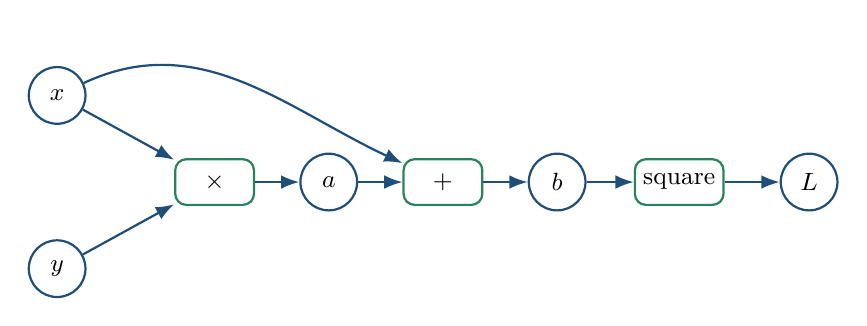
\begin{tikzpicture}
\node[var] (x) at (0,1.1) {$x$};
\node[var] (y) at (0,-1.1) {$y$};

\node[op]  (mul) at (2.0,0) {$\times$};
\node[var] (a) at (3.45,0) {$a$};

\node[op]  (add) at (4.9,0) {$+$};
\node[var] (b) at (6.35,0) {$b$};

\node[op]  (sq) at (7.9,0) {square};
\node[var] (L) at (9.55,0) {$L$};

\draw[arr] (x) -- (mul);
\draw[arr] (y) -- (mul);
\draw[arr] (mul) -- (a);
\draw[arr] (a) -- (add);
\draw[arr] (x) to[out=25,in=155] (add);
\draw[arr] (add) -- (b);
\draw[arr] (b) -- (sq);
\draw[arr] (sq) -- (L);

% \draw[barr] (L) to[bend left=45] node[above] {$\bar b$} (b);
% \draw[barr] (b) to[bend left=45] node[above] {$\bar a$} (a);
% \draw[barr] (a) to[bend left=45] node[above] {$\bar x,\bar y$} (x);

% Backward: square -> b
% \draw[barr]
%     (L) to[bend right=28]
%     node[below] {$\bar b$}
%     (b);

% % Backward: add -> a
% \draw[barr]
%     (b) to[bend right=28]
%     node[below] {$\bar a$}
%     (a);

% % Backward: add -> x (direct path)
% \draw[barr]
%     (b) to[out=145,in=-20]
%     node[below] {$\bar x_{\mathrm{direct}}$}
%     (x);

% % Backward: multiply -> x
% \draw[barr]
%     (a) to[out=150,in=-30]
%     node[below] {$\bar x_{\mathrm{via}\ a}$}
%     (x);

% % Backward: multiply -> y
% \draw[barr]
%     (a) to[out=210,in=30]
%     node[below] {$\bar y$}
%     (y);
\end{tikzpicture}
}



\vspace{0.35cm}

Forward computes values.  
Backward computes sensitivities.
\end{frame}



% ----------------------
\begin{frame}[t]{Backward pass overview}
\centering
\resizebox{0.82\textwidth}{!}{
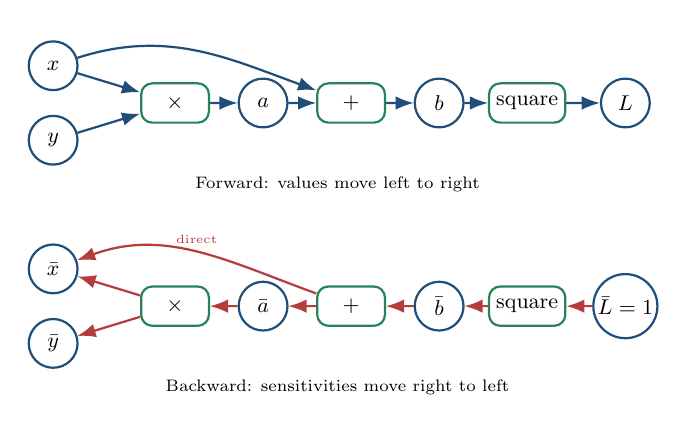
\begin{tikzpicture}[scale=0.86, transform shape]

% Forward row
\node[var] (x) at (0,1.0) {$x$};
\node[var] (y) at (0,-0.1) {$y$};
\node[op]  (mul) at (1.8,0.45) {$\times$};
\node[var] (a) at (3.1,0.45) {$a$};
\node[op]  (add) at (4.4,0.45) {$+$};
\node[var] (b) at (5.7,0.45) {$b$};
\node[op]  (sq) at (7.0,0.45) {square};
\node[var] (L) at (8.45,0.45) {$L$};

\draw[arr] (x) -- (mul);
\draw[arr] (y) -- (mul);
\draw[arr] (mul) -- (a);
\draw[arr] (a) -- (add);
\draw[arr] (x) to[out=18,in=160] (add);
\draw[arr] (add) -- (b);
\draw[arr] (b) -- (sq);
\draw[arr] (sq) -- (L);

\node at (4.2,-0.75) {\scriptsize Forward: values move left to right};

% Backward row
\node[var] (xb) at (0,-2.0) {$\bar{x}$};
\node[var] (yb) at (0,-3.1) {$\bar{y}$};
\node[op]  (mulb) at (1.8,-2.55) {$\times$};
\node[var] (ab) at (3.1,-2.55) {$\bar{a}$};
\node[op]  (addb) at (4.4,-2.55) {$+$};
\node[var] (bb) at (5.7,-2.55) {$\bar{b}$};
\node[op]  (sqb) at (7.0,-2.55) {square};
\node[var] (Lb) at (8.45,-2.55) {$\bar{L}=1$};

\draw[barr] (Lb) -- (sqb);
\draw[barr] (sqb) -- (bb);
\draw[barr] (bb) -- (addb);
\draw[barr] (addb) -- (ab);
\draw[barr] (addb) to[out=160,in=20] node[above] {\tiny direct} (xb);
\draw[barr] (ab) -- (mulb);
\draw[barr] (mulb) -- (xb);
\draw[barr] (mulb) -- (yb);

\node at (4.2,-3.75) {\scriptsize Backward: sensitivities move right to left};

\end{tikzpicture}
}
\end{frame}
% ----------------

\begin{frame}[t]{Backward pass starts at the loss}
Every backward pass begins with:

\[
\boxed{
\adj{L}
=
\grad{L}{L}
=
1
}
\]

Why?

\[
L
\]

changes one-for-one with itself.

This value \(1\) is the seed of reverse-mode autodiff.
\end{frame}

\begin{frame}[t]{Backward through square}
Forward:

\[
L=b^2
\]

Local derivative:

\[
\grad{L}{b}=2b
\]

Since \(b=8\):

\[
\grad{L}{b}=16
\]

Therefore:

\[
\adj{b}
=
\adj{L}(2b)
=
1(16)
=
16
\]
\end{frame}

\begin{frame}[t]{Backward through addition}
Forward:

\[
b=a+x
\]

Local derivatives:

\[
\grad{b}{a}=1,
\qquad
\grad{b}{x}=1
\]

We already know:

\[
\adj{b}=16
\]

\begin{columns}[T]
\column{0.46\textwidth}
\begin{block}{Gradient to \(a\)}
\[
\adj{a}=16(1)=16
\]
\end{block}

\column{0.46\textwidth}
\begin{block}{Direct gradient to \(x\)}
\[
\adj{x}_{\text{direct}}=16(1)=16
\]
\end{block}
\end{columns}
\end{frame}

\begin{frame}[t]{Backward through multiplication}
Forward:

\[
a=xy
\]

Local derivatives at \(x=2,\;y=3\):

\[
\grad{a}{x}=y=3,
\qquad
\grad{a}{y}=x=2
\]

We have:

\[
\adj{a}=16
\]

\begin{columns}[T]
\column{0.46\textwidth}
\begin{block}{Gradient to \(x\)}
\[
\adj{x}_{a}=16(3)=48
\]
\end{block}

\column{0.46\textwidth}
\begin{block}{Gradient to \(y\)}
\[
\adj{y}=16(2)=32
\]
\end{block}
\end{columns}
\end{frame}

\begin{frame}[t]{The crucial rule: gradients accumulate}
There are two paths from \(x\) to \(L\):

\[
x\rightarrow a\rightarrow b\rightarrow L
\]

and

\[
x\rightarrow b\rightarrow L
\]

Therefore:

\[
\grad{L}{x}
=
\grad{L}{x}\bigg|_{\text{via }a}
+
\grad{L}{x}\bigg|_{\text{direct}}
\]

\[
=48+16
\]

\[
\boxed{\grad{L}{x}=64}
\]
\end{frame}

\begin{frame}[t]{Final gradients}
For:

\[
L=(xy+x)^2
\]

at:

\[
x=2,\qquad y=3
\]

reverse-mode autodiff gives:

\[
\boxed{\grad{L}{x}=64}
\]

\[
\boxed{\grad{L}{y}=32}
\]

\vfill

The graph needed only local derivatives and the chain rule.
\end{frame}

\begin{frame}[t]{Full backward pass as a table}
\centering
\small

\begin{tabular}{c c c}
\toprule
Node & Rule & Gradient \\
\midrule
\(L\) & \(\adj{L}=1\) & \(1\) \\
\(b\) & \(\adj{b}=\adj{L}(2b)\) & \(16\) \\
\(a\) & \(\adj{a}=\adj{b}(1)\) & \(16\) \\
\(x\), direct & \(\adj{x}\mathrel{+}=\adj{b}(1)\) & \(16\) \\
\(x\), via \(a\) & \(\adj{x}\mathrel{+}=\adj{a}y\) & \(48\) \\
\(y\) & \(\adj{y}\mathrel{+}=\adj{a}x\) & \(32\) \\
\bottomrule
\end{tabular}

\vspace{0.35cm}

\[
\boxed{
\adj{x}=64,\qquad
\adj{y}=32
}
\]
\end{frame}

\begin{frame}[t]{Why do we use \(+=\) during backward?}
Suppose a node \(x\) feeds several later operations.

Then:

\[
\grad{L}{x}
=
\sum_i
\grad{L}{v_i}
\grad{v_i}{x}
\]

Every path contributes to the final gradient.

Conceptually, autodiff performs:

\[
\boxed{
x.\text{grad}
\mathrel{+}=
\text{gradient arriving from each child}
}
\]

This is called \textbf{gradient accumulation}.
\end{frame}

\begin{frame}[t]{Example 2: a branch-heavy graph}
Consider:

\[
u=x^2,
\qquad
v=3x
\]

\[
s=u+v
\]

\[
L=s^2
\]

For:

\[
x=2
\]

the forward values are:

\[
u=4,\qquad
v=6,\qquad
s=10,\qquad
L=100
\]
\end{frame}

\begin{frame}[t]{Example 2 graph}
\centering

\resizebox{0.69\textwidth}{!}{
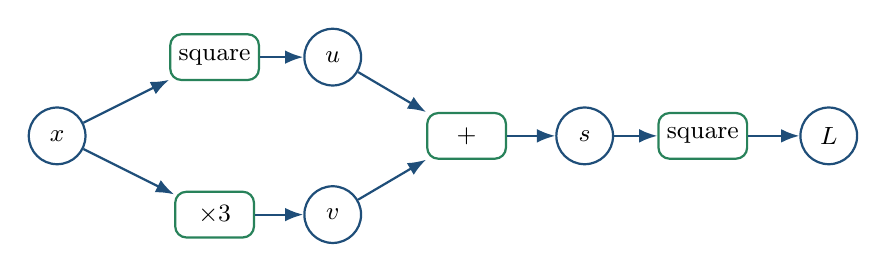
\begin{tikzpicture}
\node[var] (x) at (0,0) {$x$};

\node[op] (sq1) at (2,1) {square};
\node[var] (u) at (3.5,1) {$u$};

\node[op] (mul) at (2,-1) {$\times 3$};
\node[var] (v) at (3.5,-1) {$v$};

\node[op] (add) at (5.2,0) {$+$};
\node[var] (s) at (6.7,0) {$s$};

\node[op] (sq2) at (8.2,0) {square};
\node[var] (L) at (9.8,0) {$L$};

\draw[arr] (x) -- (sq1);
\draw[arr] (sq1) -- (u);
\draw[arr] (u) -- (add);

\draw[arr] (x) -- (mul);
\draw[arr] (mul) -- (v);
\draw[arr] (v) -- (add);

\draw[arr] (add) -- (s);
\draw[arr] (s) -- (sq2);
\draw[arr] (sq2) -- (L);
\end{tikzpicture}
}

\vspace{0.35cm}

The forward pass splits at \(x\).

The backward pass merges gradients at \(x\).
\end{frame}

\begin{frame}[t]{Example 2: backward to the branches}
Start with:

\[
\adj{L}=1
\]

Since:

\[
L=s^2
\]

we get:

\[
\adj{s}=2s=20
\]

Since:

\[
s=u+v
\]

the gradient goes to both branches:

\[
\boxed{
\adj{u}=20,
\qquad
\adj{v}=20
}
\]
\end{frame}

\begin{frame}[t]{Example 2: merge the gradients}
For the first branch:

\[
u=x^2
\]

\[
\adj{x}_u
=
20(2x)
=
20(4)
=
80
\]

For the second branch:

\[
v=3x
\]

\[
\adj{x}_v
=
20(3)
=
60
\]

Therefore:

\[
\boxed{
\adj{x}=80+60=140
}
\]
\end{frame}

\begin{frame}[t]{Parameter sharing is the same idea}
Suppose one weight is reused:

\[
y=wx_1+wx_2
\]

and:

\[
L=y^2
\]

The same parameter \(w\) participates twice.

Therefore:

\[
\grad{L}{w}
=
\grad{L}{w}\bigg|_{wx_1}
+
\grad{L}{w}\bigg|_{wx_2}
\]

This happens with shared embeddings, recurrent networks, tied weights, and reused modules.
\end{frame}

\begin{frame}[t]{Residual connections and gradient flow}
A residual block computes:

\[
y=F(x)+x
\]

Therefore:

\[
\grad{y}{x}=F'(x)+1
\]

\centering

\resizebox{0.58\textwidth}{!}{
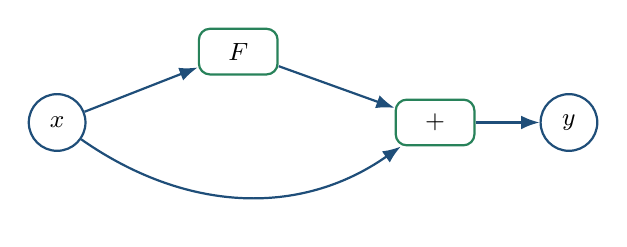
\begin{tikzpicture}
\node[var] (x) at (0,0) {$x$};
\node[op] (F) at (2.3,0.9) {$F$};
\node[op] (add) at (4.8,0) {$+$};
\node[var] (y) at (6.5,0) {$y$};

\draw[arr] (x) -- (F);
\draw[arr] (F) -- (add);
\draw[arr] (x) to[out=-35,in=-145] (add);
\draw[arr] (add) -- (y);
\end{tikzpicture}
}

\vspace{0.25cm}

The identity branch gives a direct route for gradients.
\end{frame}

\begin{frame}[t]{Example 3: ReLU is also a graph operation}
Forward:

\[
h=\operatorname{ReLU}(z)
\]

where:

\[
\operatorname{ReLU}(z)=\max(0,z)
\]

Its local derivative is:

\[
\grad{h}{z}
=
\begin{cases}
1, & z>0 \\
0, & z<0
\end{cases}
\]

So backward becomes:

\[
\boxed{
\adj{z}
=
\adj{h}\mathbf{1}[z>0]
}
\]
\end{frame}

\begin{frame}[t]{ReLU: forward and backward}
\centering
\small

\begin{tabular}{c c c}
\toprule
Forward input & Forward output & Backward behaviour \\
\midrule
\(z>0\) & \(h=z\) & gradient passes \\
\(z<0\) & \(h=0\) & gradient becomes zero \\
\bottomrule
\end{tabular}

\vspace{0.5cm}

For PyTorch, the derivative chosen at \(z=0\) is \(0\).

\vfill

The backward rule needs information from the forward pass.
\end{frame}



\begin{frame}[t]{What if the gradient becomes zero?}
Autodiff uses the same chain rule:

\[
\grad{L}{u}=\grad{L}{v}\grad{v}{u}
\]

If the local derivative is zero:

\[
\grad{v}{u}=0
\quad\Rightarrow\quad
\grad{L}{u}=0
\]

\vfill

\[
\boxed{
\text{The graph is still valid. It just sends zero backward.}
}
\]
\end{frame}

\begin{frame}[t]{Example: ReLU blocks one path}
Let:

\[
z=-2,\qquad h=\operatorname{ReLU}(z)=0,\qquad L=3h
\]

Then:

\[
\grad{L}{h}=3
\]

For ReLU, when \(z<0\):

\[
\grad{h}{z}=0
\]

So:

\[
\grad{L}{z}=3\cdot 0=0
\]

\vfill

The gradient does not pass through this ReLU path.
\end{frame}

\begin{frame}[t]{Zero on one path does not kill all paths}
Consider:

\[
y=\operatorname{ReLU}(x)+x,\qquad L=y^2,\qquad x=-2
\]

Then:

\[
y=-2,\qquad \grad{L}{y}=2y=-4
\]

\begin{columns}[T]
\column{0.48\textwidth}
\begin{block}{ReLU path}
\[
-4\cdot 0=0
\]
\end{block}

\column{0.48\textwidth}
\begin{block}{Identity path}
\[
-4\cdot 1=-4
\]
\end{block}
\end{columns}

\vfill

\[
\boxed{\grad{L}{x}=0-4=-4}
\]
\end{frame}

\begin{frame}[fragile,t]{PyTorch: zero gradient}
\begin{lstlisting}[language=Python]
import torch

x = torch.tensor(-2.0, requires_grad=True)

h = torch.relu(x)
L = 3 * h

L.backward()

print(h)       # tensor(0., grad_fn=<ReluBackward0>)
print(x.grad)  # tensor(0.)
\end{lstlisting}

\vfill

\[
x.\texttt{grad}=0
\]

means \(x\) was tracked, but the derivative was zero.
\end{frame}

\begin{frame}[fragile,t]{Zero gradient vs no gradient}
\begin{lstlisting}[language=Python]
x = torch.tensor(2.0, requires_grad=True)
y = torch.tensor(3.0, requires_grad=True)

z = x.detach() * y
L = z ** 2
L.backward()

print(x.grad)  # None
print(y.grad)  # tensor(24.)
\end{lstlisting}

\vfill

\[
x.\texttt{grad}=0
\quad\neq\quad
x.\texttt{grad}=\texttt{None}
\]

Zero means tracked but derivative is zero.  
None means not connected to the graph.
\end{frame}

\begin{frame}[t]{From scalar nodes to tensor nodes}
Real neural networks operate on tensors.

For example:

\[
x\in\mathbb{R}^{d}
\]

\[
W\in\mathbb{R}^{m\times d}
\]

\[
z=Wx+b
\]

The graph idea does not change.

The local derivatives become matrices called:

\[
\boxed{\text{Jacobians}}
\]
\end{frame}

\begin{frame}[t]{Why autodiff does not build giant Jacobians}
Suppose:

\[
y=f(x)
\]

with Jacobian:

\[
J=\grad{y}{x}
\]

In reverse mode, we receive an upstream gradient:

\[
\adj{y}
\]

and need:

\[
\boxed{
\adj{x}=J^\top\adj{y}
}
\]

This is a \textbf{vector--Jacobian product}.

Autodiff computes this product directly.
\end{frame}

\begin{frame}[t]{Linear layer computational graph}
\centering

\resizebox{0.73\textwidth}{!}{
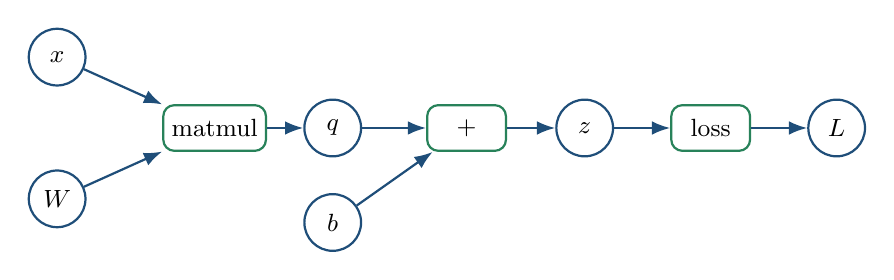
\begin{tikzpicture}
\node[var] (x) at (0,0.9) {$x$};
\node[var] (W) at (0,-0.9) {$W$};

\node[op] (mm) at (2,0) {matmul};
\node[var] (q) at (3.5,0) {$q$};

\node[var] (b) at (3.5,-1.2) {$b$};

\node[op] (add) at (5.2,0) {$+$};
\node[var] (z) at (6.7,0) {$z$};

\node[op] (loss) at (8.3,0) {loss};
\node[var] (L) at (9.9,0) {$L$};

\draw[arr] (x) -- (mm);
\draw[arr] (W) -- (mm);
\draw[arr] (mm) -- (q);
\draw[arr] (q) -- (add);
\draw[arr] (b) -- (add);
\draw[arr] (add) -- (z);
\draw[arr] (z) -- (loss);
\draw[arr] (loss) -- (L);
\end{tikzpicture}
}

\vspace{0.35cm}

\[
q=Wx,\qquad z=q+b
\]
\end{frame}

\begin{frame}[t]{Backward rules for a linear layer}
Suppose the backward pass gives:

\[
g=\grad{L}{z}
\]

For:

\[
z=Wx+b
\]

the local backward rules are:

\begin{columns}[T]
\column{0.31\textwidth}
\begin{block}{Input}
\[
\boxed{
\grad{L}{x}=W^\top g
}
\]
\end{block}

\column{0.31\textwidth}
\begin{block}{Weights}
\[
\boxed{
\grad{L}{W}=gx^\top
}
\]
\end{block}

\column{0.31\textwidth}
\begin{block}{Bias}
\[
\boxed{
\grad{L}{b}=g
}
\]
\end{block}
\end{columns}
\end{frame}

\begin{frame}[t]{Small matrix example: forward pass}
Let:

\[
W=
\begin{bmatrix}
1&2\\
3&4
\end{bmatrix},
\qquad
x=
\begin{bmatrix}
1\\
2
\end{bmatrix},
\qquad
b=
\begin{bmatrix}
0\\
1
\end{bmatrix}
\]

Then:

\[
z=Wx+b
=
\begin{bmatrix}
5\\
12
\end{bmatrix}
\]

Define:

\[
L=z_1+z_2=17
\]
\end{frame}

\begin{frame}[t]{Small matrix example: gradient to \(z\)}
Since:

\[
L=z_1+z_2
\]

we get:

\[
\grad{L}{z_1}=1,
\qquad
\grad{L}{z_2}=1
\]

Therefore:

\[
\boxed{
g=
\grad{L}{z}
=
\begin{bmatrix}
1\\
1
\end{bmatrix}
}
\]

This gradient is now passed through the linear operation.
\end{frame}

\begin{frame}[t]{Small matrix example: gradient to \(x\)}
Use:

\[
\grad{L}{x}=W^\top g
\]

Then:

\[
W^\top=
\begin{bmatrix}
1&3\\
2&4
\end{bmatrix}
\]

Therefore:

\[
\grad{L}{x}
=
\begin{bmatrix}
1&3\\
2&4
\end{bmatrix}
\begin{bmatrix}
1\\
1
\end{bmatrix}
=
\boxed{
\begin{bmatrix}
4\\
6
\end{bmatrix}
}
\]
\end{frame}

\begin{frame}[t]{Small matrix example: gradient to \(W\)}
Use:

\[
\grad{L}{W}
=
gx^\top
\]

We have:

\[
g=
\begin{bmatrix}
1\\
1
\end{bmatrix},
\qquad
x^\top=
\begin{bmatrix}
1&2
\end{bmatrix}
\]

Therefore:

\[
\grad{L}{W}
=
\boxed{
\begin{bmatrix}
1&2\\
1&2
\end{bmatrix}
}
\]
\end{frame}

\begin{frame}[t]{Forward mode vs reverse mode}
For:

\[
f:\mathbb{R}^{n}\rightarrow\mathbb{R}^{m}
\]

the Jacobian has shape:

\[
m\times n
\]

\begin{columns}[T]
\column{0.46\textwidth}
\begin{block}{Forward mode}
Efficiently computes:

\[
Jv
\]

Useful when:

\[
n\ll m
\]
\end{block}

\column{0.46\textwidth}
\begin{block}{Reverse mode}
Efficiently computes:

\[
v^\top J
\]

Useful when:

\[
m\ll n
\]
\end{block}
\end{columns}
\end{frame}

\begin{frame}[t]{Why deep learning uses reverse mode}
A neural network can have:

\[
n=10^6,\;10^9,\;\text{or more parameters}
\]

but training normally ends with:

\[
L\in\mathbb{R}
\]

Therefore:

\[
f:\mathbb{R}^{n}\rightarrow\mathbb{R}
\]

One reverse traversal can compute:

\[
\boxed{\nabla_\theta L}
\]

for all parameters.
\end{frame}

\begin{frame}[t]{What an autodiff engine records}
For:

\[
a=xy,
\qquad
b=a+x,
\qquad
L=b^2
\]

the engine records something like:

\small

\begin{center}
\begin{tabular}{c c}
\toprule
Forward operation & Backward rule \\
\midrule
\(a=xy\)
&
\(\adj{x}{+}=\adj{a}y,\;
  \adj{y}{+}=\adj{a}x\)
\\[0.15cm]
\(b=a+x\)
&
\(\adj{a}{+}=\adj{b},\;
  \adj{x}{+}=\adj{b}\)
\\[0.15cm]
\(L=b^2\)
&
\(\adj{b}{+}=\adj{L}(2b)\)
\\
\bottomrule
\end{tabular}
\end{center}
\end{frame}

\begin{frame}[fragile,t]{Tape-like pseudocode}
\begin{lstlisting}[language=Python]
# Forward
a = multiply(x, y)
b = add(a, x)
L = square(b)

# Start backward
L.grad = 1

# Reverse graph order
b.grad += L.grad * 2 * b

a.grad += b.grad
x.grad += b.grad

x.grad += a.grad * y
y.grad += a.grad * x
\end{lstlisting}
\end{frame}

\begin{frame}[t]{Dynamic computational graphs}
PyTorch builds the computational graph while the forward code executes.

\[
x
\rightarrow
\text{operation 1}
\rightarrow
\text{operation 2}
\rightarrow
L
\]

The graph records the operations that were actually executed.

\vfill

This is why ordinary Python control flow can participate in PyTorch models.
\end{frame}

\begin{frame}[fragile,t]{The same example in PyTorch}
\begin{lstlisting}[language=Python]
import torch

x = torch.tensor(2.0, requires_grad=True)
y = torch.tensor(3.0, requires_grad=True)

a = x * y
b = a + x
L = b ** 2

L.backward()

print(x.grad)
print(y.grad)
\end{lstlisting}

Output:

\begin{lstlisting}
tensor(64.)
tensor(32.)
\end{lstlisting}
\end{frame}

\begin{frame}[fragile,t]{PyTorch exposes parts of the graph}
For intermediate tensors:

\begin{lstlisting}[language=Python]
print(a.grad_fn)
print(b.grad_fn)
print(L.grad_fn)
\end{lstlisting}

Typical output resembles:

\begin{lstlisting}
<MulBackward0>
<AddBackward0>
<PowBackward0>
\end{lstlisting}

These objects represent backward operations associated with the forward graph.
\end{frame}

\begin{frame}[t]{What does \texttt{requires\_grad=True} mean?}
When we write:

\[
\texttt{requires\_grad=True}
\]

we tell PyTorch:

\begin{quote}
Track operations involving this tensor because derivatives may be needed later.
\end{quote}

This tracking has a cost:

\begin{itemize}
    \item extra graph objects,
    \item saved activations,
    \item additional memory.
\end{itemize}
\end{frame}

\begin{frame}[t]{Leaf tensors and intermediate tensors}
Consider:

\[
x,y
\rightarrow
a
\rightarrow
b
\rightarrow
L
\]

Usually:

\begin{itemize}
    \item \(x\) and \(y\) are \textbf{leaf tensors},
    \item \(a,b,L\) are \textbf{intermediate tensors}.
\end{itemize}

PyTorch normally stores accumulated gradients in:

\[
x.\texttt{grad},
\qquad
y.\texttt{grad}
\]

for leaf tensors that require gradients.
\end{frame}

\begin{frame}[t]{Why training uses more memory than inference}
Backward often needs forward values.

Example:

\[
y=x^2
\]

The backward rule uses:

\[
2x
\]

so \(x\) must still be available.

Deep networks save many intermediate activations during forward.

Therefore:

\[
\boxed{
\text{training memory}
>
\text{inference memory}
}
\]
\end{frame}

\begin{frame}[t]{Gradient checkpointing}
Standard training:

\[
\text{store many activations}
\]

uses more memory.

Gradient checkpointing stores fewer activations and recomputes some of them during backward.

Therefore it trades:

\[
\boxed{
\text{extra computation}
\quad\leftrightarrow\quad
\text{lower memory usage}
}
\]
\end{frame}

\begin{frame}[t]{Autodiff is not numerical differentiation}
Numerical differentiation uses:

\[
f'(x)
\approx
\frac{f(x+\epsilon)-f(x)}{\epsilon}
\]

It requires extra function evaluations and depends on \(\epsilon\).

Autodiff instead differentiates the primitive operations used to compute \(f\).

\[
\boxed{
\text{Autodiff uses the chain rule, not finite differences.}
}
\]
\end{frame}

\begin{frame}[t]{Autodiff is not symbolic differentiation}
Symbolic differentiation manipulates mathematical expressions.

For example:

\[
f(x)=(x^2+3x)^5
\]

could produce:

\[
f'(x)=5(x^2+3x)^4(2x+3)
\]

Autodiff does not need to create this expression.

\vfill

It evaluates local derivative rules along the executed graph.
\end{frame}

% \begin{frame}[t]{In-class exercise}
% Let:

% \[
% a=x+y
% \]

% \[
% b=xy
% \]

% \[
% L=ab
% \]

% with:

% \[
% x=2,
% \qquad
% y=3
% \]

% Find:

% \[
% \boxed{
% \grad{L}{x}
% \qquad\text{and}\qquad
% \grad{L}{y}
% }
% \]

% Hint: both \(x\) and \(y\) are used by two branches.
% \end{frame}

% \begin{frame}[t]{In-class exercise: forward pass}
% For:

% \[
% x=2,
% \qquad
% y=3
% \]

% we get:

% \[
% a=x+y=5
% \]

% \[
% b=xy=6
% \]

% \[
% L=ab=30
% \]

% Now start backward with:

% \[
% \adj{L}=1
% \]
% \end{frame}

% \begin{frame}[t]{In-class exercise: backward pass}
% Since:

% \[
% L=ab
% \]

% we have:

% \[
% \adj{a}=b=6,
% \qquad
% \adj{b}=a=5
% \]

% For \(x\):

% \[
% \adj{x}
% =
% 6(1)+5(3)
% =
% \boxed{21}
% \]

% For \(y\):

% \[
% \adj{y}
% =
% 6(1)+5(2)
% =
% \boxed{16}
% \]
% \end{frame}

\begin{frame}[t]{The mental model to keep}
When you see:

\[
\texttt{loss.backward()}
\]

think:

\begin{enumerate}
    \item Set the loss gradient to \(1\).
    \item Visit operations in reverse dependency order.
    \item Multiply incoming gradient by local derivative.
    \item Send the result to each input.
    \item Add gradients when multiple paths reach the same value.
\end{enumerate}
\end{frame}

\begin{frame}[t]{Three ideas explain almost everything}
\begin{block}{1. Computational graph}
Records operations and dependencies.
\end{block}

\begin{block}{2. Chain rule}
Propagates sensitivities through each operation.
\end{block}

\begin{block}{3. Gradient accumulation}
Adds contributions from multiple paths.
\end{block}

\vfill

Together, these give reverse-mode automatic differentiation.
\end{frame}

\begin{frame}[t]{Final takeaway}
\[
\boxed{
\text{Computational graph}
=
\text{operations}
+
\text{dependencies}
}
\]

\vspace{0.25cm}

\[
\boxed{
\text{Autodiff}
=
\text{local derivatives}
+
\text{chain rule}
+
\text{gradient accumulation}
}
\]

\vspace{0.25cm}

\[
\boxed{
\text{Backpropagation}
=
\text{reverse-mode autodiff applied to a neural network}
}
\]
\end{frame}

\begin{frame}[t]{Next: visualising this in PyTorch}
In the notebook, we can build the same ideas step by step:

\begin{enumerate}
    \item manually implement scalar backpropagation,
    \item recreate it using PyTorch,
    \item inspect \texttt{grad\_fn},
    \item retain gradients on intermediate tensors,
    \item visualise the graph,
    \item demonstrate branch gradient accumulation,
    \item inspect ReLU backward behaviour,
    \item manually verify a linear-layer gradient.
\end{enumerate}
\end{frame}

\end{document}